\documentclass[12pt, a4paper]{article}

\usepackage[medium]{titlesec}
\usepackage{graphicx}
\usepackage{caption}
\usepackage{amsmath}
\usepackage{amsthm}
\usepackage[legalpaper, portrait, margin=1.2in]{geometry}
\usepackage{wrapfig}
\usepackage{varwidth}
\usepackage{listings}
\usepackage{amssymb}
\usepackage{enumitem}
\usepackage{bm}
\usepackage{enumitem}

\allowdisplaybreaks  % will allow page break in align environment

\begin{document}
	
	\setlength{\parindent}{0pt}
	\captionsetup{justification=centering}
	\lstset{
		showstringspaces=false
	}
	
	
	\begin{titlepage}
		\LARGE
		\textbf{7.5}
		\begin{center}
			\vspace*{7cm}
			
			\LARGE
			\textbf{Mathematical Methods}
			\\
			\vspace{1cm}
			\textbf{Pad\'e Approximants}
			
			\vspace{0.5cm}
		\end{center}
	\end{titlepage}

\section{Introduction}	
	
\subsubsection*{Programming Task: Writing Programs A and B}

The programs written for this task can be found on pages \pageref{Program_A} and \
\pageref{Program_B}. From the numpy package in Python, I use the \texttt{lstsq} function \
as an equivalent of \texttt{mldivide} from Matlab. I first tested Program A for basic \
functions such as f(x) = 0 with different values of L and M. Then I carried out testing \
with more complex functions such as f(x) = sin(x) and confirming the $O(x^{L+M+1})$ \
accuracy via polynomial division of the results.


\subsubsection*{Question 1}

NEED TO TAKE M = L + 1 SOMEWHERE IN THIS PROJECT. IN QUESTION 4? - WHAT IS THE DETERMINANT IN PROGRAM A HERE?
- COULD IT AFFECT ERROR IN QUESTION 3?

Using the binomial expansion, we obtain,
\begin{flalign*}
	f_{1}(x) = 1 + \frac{x}{2} - \frac{x^{2}}{8} + \frac{x^{3}}{16} &&
\end{flalign*}
with the following formula for the coefficients,
\begin{flalign*}
	c_{0} = 1, \quad c_{1} = \frac{1}{2}, \quad c_{k} = \frac{ (-1)^{k-1}(2k-3)! }{ 2^{2k-2}k!(k-2)! } \text{ for } \ 
	k \geq 1. &&
\end{flalign*}

The radius of convergence can be found via the ratio test.
\begin{flalign*}
	\text{Radius} & = \lim_{k \to \infty} \left| \frac{ c_{k} }{ c_{k+1} } \right| &&\\
	& = \lim_{k \to \infty}\left| \frac{ (2k-1)(2k-2) }{ 4(k+1)(k-1) } \right| &&\\
	& = 1
\end{flalign*}
THIS MEANS that the Pad\'e APPROXIMANT will only be useful within the disk of radius 1 \ 
centred at 0 in the complex plane. Also, the further from 0 you go, the more terms of \ 
the power series are required for a precise result. Therefore, approximants with a \ 
lower value of L+M+1 become much less useful in these cases.
\\

Taking $x = 1$ in the power series, we obtain $\sum_{k = 0}^{\infty}c_{k}$. Since this converges, the \
sequence of partial sums $\sum_{k = 0}^{N}c_{k}$ converges. This convergence is illustrated in Figure\ 
\ref{q1_fig1}.

\vspace{0.3cm}
\begin{minipage}{\textwidth}
	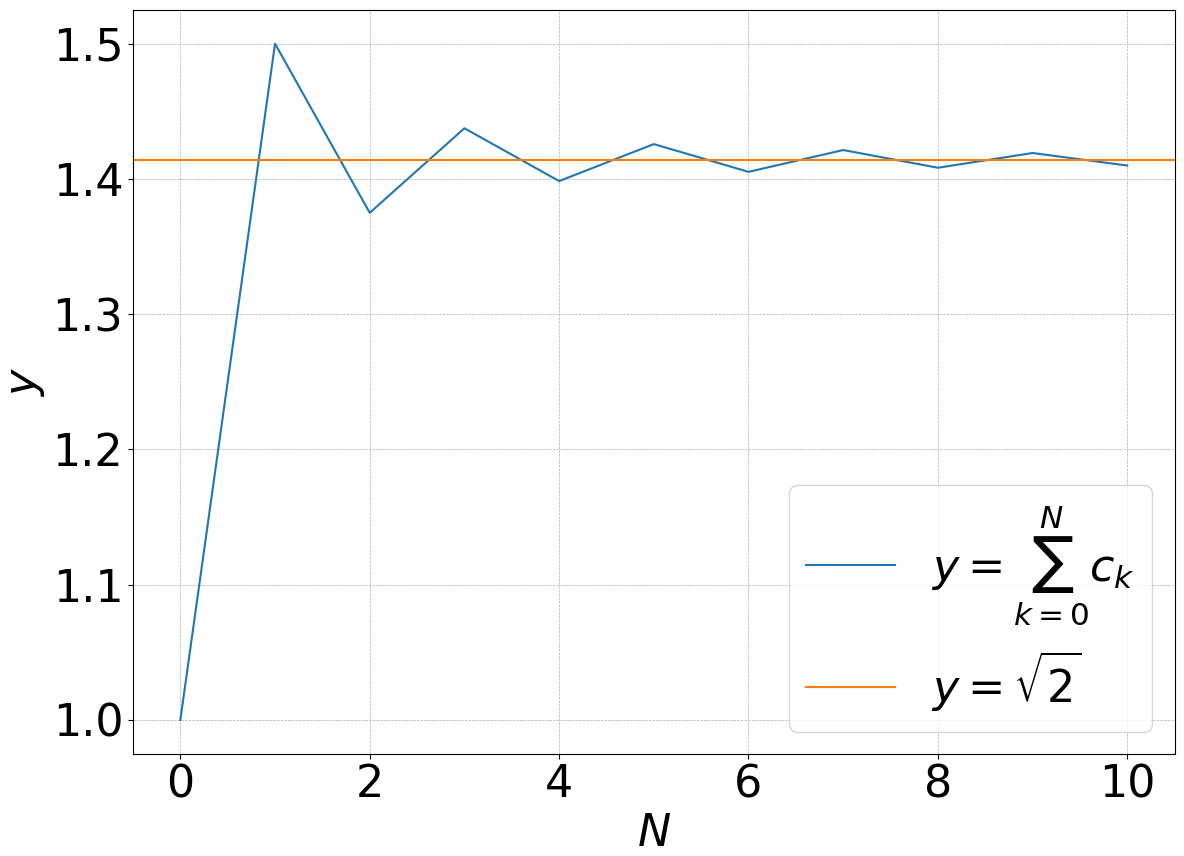
\includegraphics[width=\linewidth]{q1_fig1}
	\captionof{figure}{Line graph of partial sums}
	\label{q1_fig1}
\end{minipage}
\vspace{0.1cm}

We notice that the partial sums oscillate above and below $\sqrt{2}$, with the error getting smaller\
as $k$ increases. \\

We use the Lagrange form of the remainder for a Taylor expansion to estimate the error of the \
partial sum as an estimate of $\sqrt{2}$. The remainder at $x = 1$ will be,
\begin{flalign*}
	R_{N}(1) = \frac{ f_{1}^{(N+1)}(\xi) }{ (N+1)! } &&
\end{flalign*}
for some real number $\xi$ between 0 and 1 and following simplifications, we have,
\begin{flalign*}
	|R_{N}(1)|  = \frac{ (2N-1)! }{ 2^{2N}(N-1)!(N+1)! } (1+\xi)^{ -N + \frac{1}{2} } &&
\end{flalign*}
\\
Using the function \texttt{find\textunderscore xi} in the program on page \pageref{Question_1}, \ 
we find that $\xi$ is small and decreases as $N$ increases. For example, for $N = 3$, $\xi$ = 0.230; \ 
for $N = 10$, $\xi = 0.0681$ and for $N = 50$, $\xi = 0.0138$. Then the \
\texttt{print\textunderscore xi\textunderscore factor} also in the program on page \pageref{Question_1} \
can be used to show that for $N < 80$,  $ 0.5 \leq (1+\xi)^{ -N + \frac{1}{2} } \leq 0.7$. Hence, \
we have,
\begin{flalign}
	R_{N}(1)  &\leq 0.7 \cdot \frac{ (2N-1)! }{ 2^{2N}(N-1)!(N+1)! } && \nonumber \\
	&= 0.7 \cdot \frac{1 \cdot 3 \cdot 5 \cdot ... \cdot (2N - 1) }{ 2 \cdot 4 \cdot 6 \cdot ... \cdot 2N} \
	\cdot \frac{1}{2N+2} \label{error_eq}
\end{flalign}
We prove the following lemma:
\begin{flalign*}
	\frac{1 \cdot 3 \cdot 5 \cdot ... \cdot (2N - 1) }{ 2 \cdot 4 \cdot 6 \cdot ... \cdot 2N} \leq \ 
	\frac{1}{\sqrt{2N}}  && \\
	\text{Proof: } \left( \frac{1 \cdot 3 \cdot 5 \cdot ... \cdot (2N - 1) }{ 2 \cdot 4 \cdot 6 \cdot ... \cdot 2N}\ 
	\right)^{2} &= \frac{1 \cdot 1}{2 \cdot 2} \ 
	\cdot \frac{3 \cdot 3}{4 \cdot 4} ...\frac{(2N-1) \cdot (2N-1)}{2N \cdot 2N} && \\
	&= \frac{1 \cdot 3}{2 \cdot 2} \cdot \frac{3 \cdot 5}{4 \cdot 4} ... \ 
	\frac{(2N-1) }{(2N)^{2}} && \\
	&\leq \frac{2N-1}{(2N)^{2}} \text{ ~since~ } (n-1)(n+1) = n^{2}-1 \leq n^{2} && \\
	&\leq 1/2N ~~~~~~~~~~~~~~~~~~~~~~~~~~~~~~~~~~~~~~~~~~~~~~~~~~~ \qed
\end{flalign*}
Applying the lemma to (\ref{error_eq}), we obtain the following overestimate for the error as $N$ increases:
\begin{flalign}
	|R_{N}(1)|  \approx \frac{ 0.7 }{ (2N+2)\sqrt{2N} } \label{q1_eq2}
\end{flalign}
Figure \ref{q1_fig2} illustrates this as an error bound. We can see that this gives an accurate 
approximation of the error.

\vspace{0.3cm}
\begin{minipage}{\textwidth}
	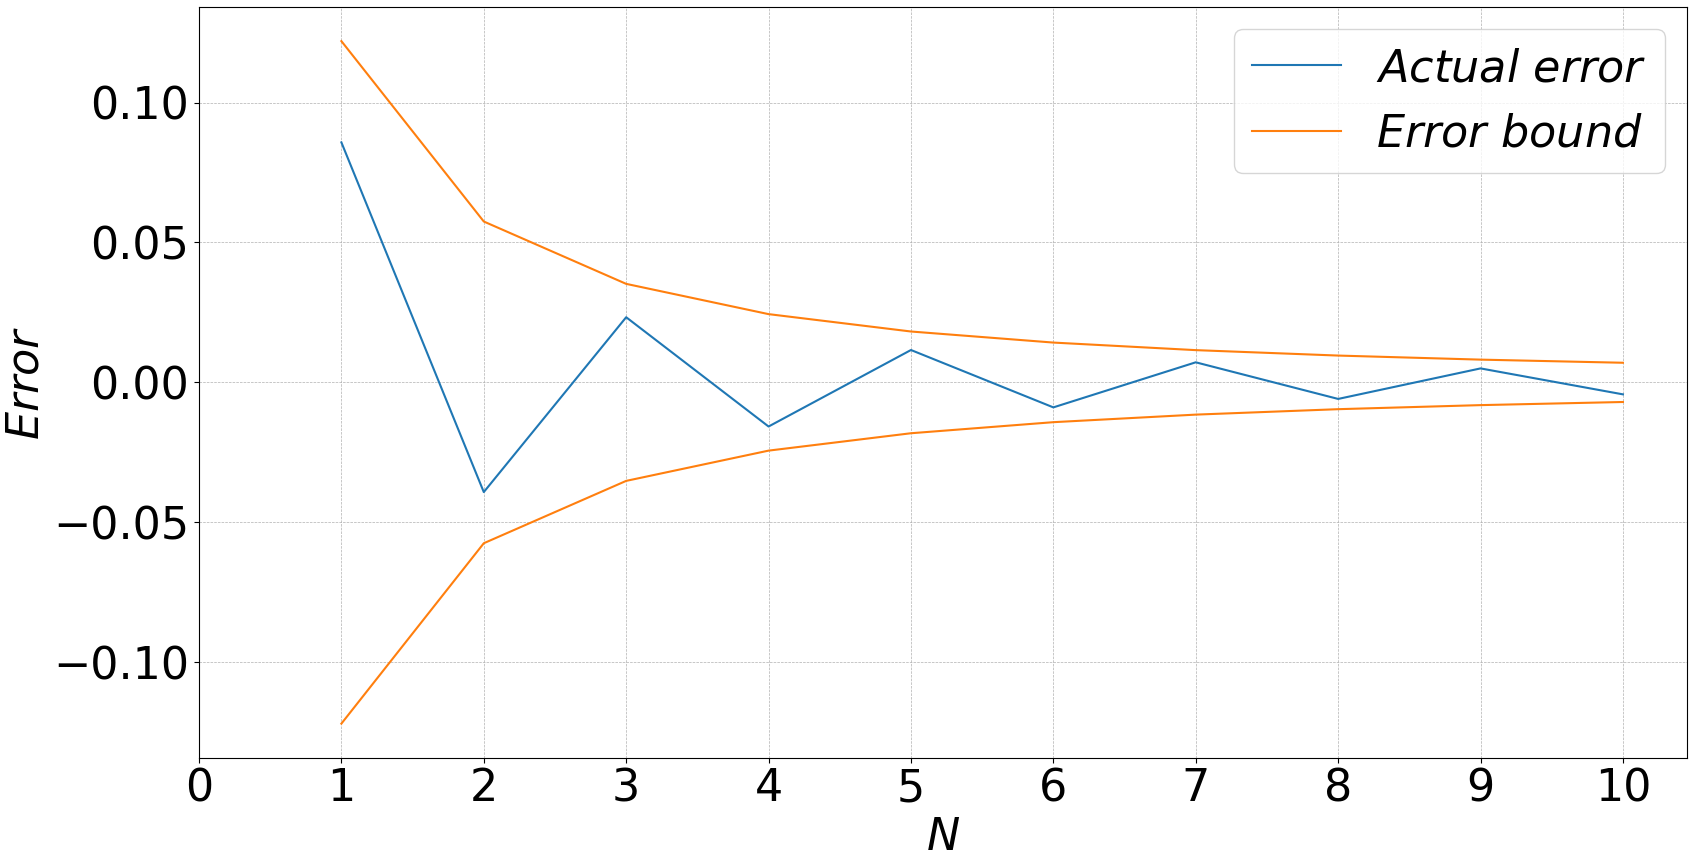
\includegraphics[width=\linewidth]{q1_fig2}
	\captionof{figure}{Actual error and estimated erro of the partial sum as an estimate of $\sqrt{2}$}
	\label{q1_fig2}
\end{minipage}
\vspace{0.1cm}

We know $(1+\xi)^{-N + \frac{1}{2}}$ is relatively unchanged when $N$ is increased by $1$. Thus taking \
the ratio of $R_{N}(1)$ and $R_{N+1}(1)$ shows that incrementing $N$ by $1$ decreases the error by \
almost exactly $\frac{ 2N+1 }{ 2N+4 }$. Hence the larger N is, the less the percentage decrease of error \
is for increasing N.


\subsubsection*{Question 2}

It is now much more difficult to obtain a theoretical result for the error, so we investigate $R_{L,L}(1)$\
as an estimate of $\sqrt{2}$ numercially. The results in the table below show the error of the approximant\
for different values of $L$.
\vspace{0.3cm}

\begin{minipage}{\textwidth}\centering
	\begin{tabular}{|l|l|}
	\hline
	\multicolumn{1}{|c|}{$L$} & \multicolumn{1}{c|}{Error}                  \\ \hline
	\multicolumn{1}{|c|}{0}   & \multicolumn{1}{c|}{0.41421356237309515}    \\ \hline
	\multicolumn{1}{|c|}{1}   & \multicolumn{1}{c|}{0.014213562373095234}   \\ \hline
	\multicolumn{1}{|c|}{2}   & \multicolumn{1}{c|}{0.00042045892481934466} \\ \hline
	\multicolumn{1}{|c|}{3}   & \multicolumn{1}{c|}{1.2378941142587863e-05} \\ \hline
	4                         & 3.644035522221145e-07                       \\ \hline
	5                         & 1.072704058913132e-08                       \\ \hline
	6                         & 3.1577518377901015e-10                      \\ \hline
	7                         & 9.29567534058151e-12                        \\ \hline
	8                         & 2.737809978725636e-13                       \\ \hline
	9                         & 7.993605777301127e-15                       \\ \hline
	10                        & 4.440892098500626e-16                       \\ \hline
	11                        & 2.220446049250313e-16                       \\ \hline
	12                        & 2.220446049250313e-16                       \\ \hline
	13                        & 6.661338147750939e-16                       \\ \hline
	14                        & 6.661338147750939e-16                       \\ \hline
	15                        & 2.220446049250313e-16                       \\ \hline
	\end{tabular}
\end{minipage}
\vspace{0.3cm}

\begin{minipage}{\textwidth}
	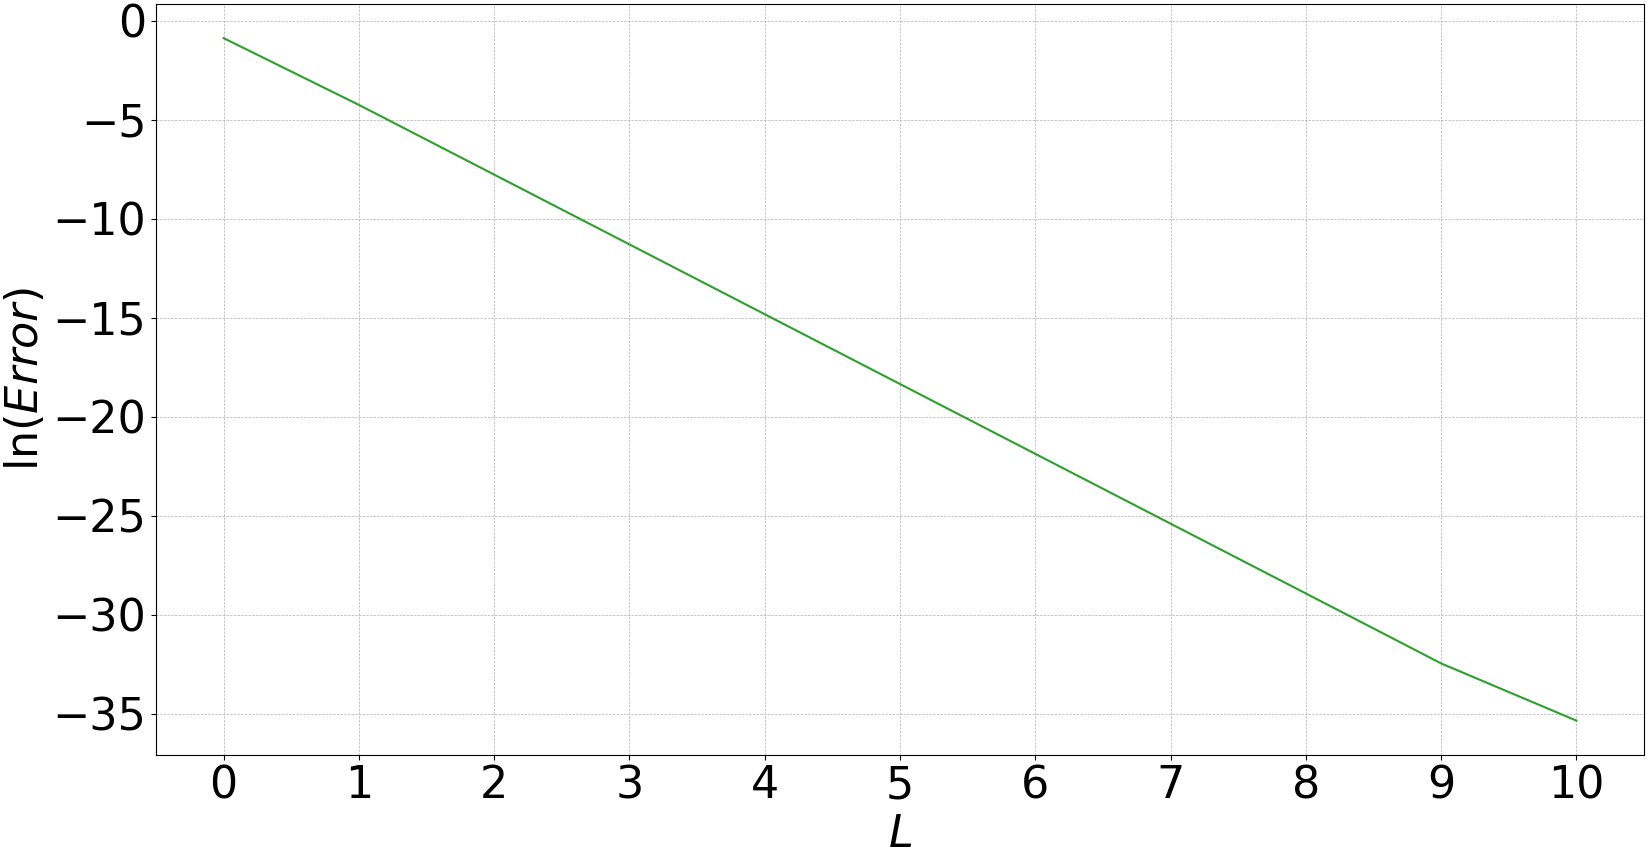
\includegraphics[width=\linewidth]{q2_fig1}
	\captionof{figure}{Plot of $L$ against $\ln(Error)$}
	\label{q2_fig1}
\end{minipage}
\vspace{0.3cm}

From Figure \ref{q2_fig1}, we see that for $L \leq 10$, the error decreases exponentially.
We observe from the table that the minimum value of the error for $L \leq 15$ is 2.220446049250313e-16.\ 
This must be true in general since this is exactly the machine precision, i.e. it is the  difference between 1.0 and\ 
the smallest 64-bit double precision floating-point value larger than 1.0. Hence, the machine precision\ 
determines the smallest error.
\\

In cases where the matrix used to solve equation (4) is non-singular, iterative improvement will make no\ 
difference since the exact solution is found so no more improvements can be made. The determinant of the\
matrix in question approaches 0 as $L$ increases. The \texttt{lstsq} function which I have used as the\ 
Python equivalent of \texttt{mldivide} finds the least-squares solution of the equation $A\mathbf{x} = \mathbf{b}$. 
Suppose for some $L$ the determinant of the matrix used to solve equation (4) were 0 and let the least\ 
squares solution for the $q_{k}$ be $\mathbf{y}$. Then $\mathbf{b}-A\mathbf{y}$ will be orthogonal to \ 
$A\mathbf{x}$ for any $\mathbf{x}$. Hence no more improvements can be made in this case either.
\\

In addition, the limit on the error is caused my the machine precision, not the solution to equation (4).\ 
Thus iterative improvement would have no effect on the minimum error.
\\

In the power series of $R_{L,L}(x)$, the first $2L+1$ terms match that of $f_{1}(x)$. The error of\ 
$R_{L,L}(1)$ is much less than the power series estimate of $\sqrt{2}$ for the same number of matching terms.\
For instance, with $L = 5$, the error of the Pad\'e approximant is $1.07 \times 10^{-8}$ while for\ 
$N=10$ the error from the partial sum is $4.28 \times 10^{-2}$. This is surprising because using the same\
amount of information, a much more accurate estimate is obtained. This can be explained by the fact that\ 
as we approach the radius of convergence the error power series expansion of $f_{1}(x)$ diverges at a\
faster rate than the error term from the power series expansion of $R_{L,L}(x)$.
\\

It is then clear that the Pad\'e approximant should be used as an estimate of $\sqrt{2}$ to specified accuracy\
in all cases. The error estimation (\ref{q1_eq2}) shows that to have an error of $2.22\times10^{-16}$, which\ 
only requires $L=11$ for the Pad\'e approximant, you would need $N$ to be close to 100,000. Even if you wanted\ 
more accuracy than this, that wouldn't be possible with 64-bit floats since $2.22\times10^{16}$ is the\ 
machine precision.


\subsubsection*{Question 3}

\begin{minipage}{\textwidth}\centering
	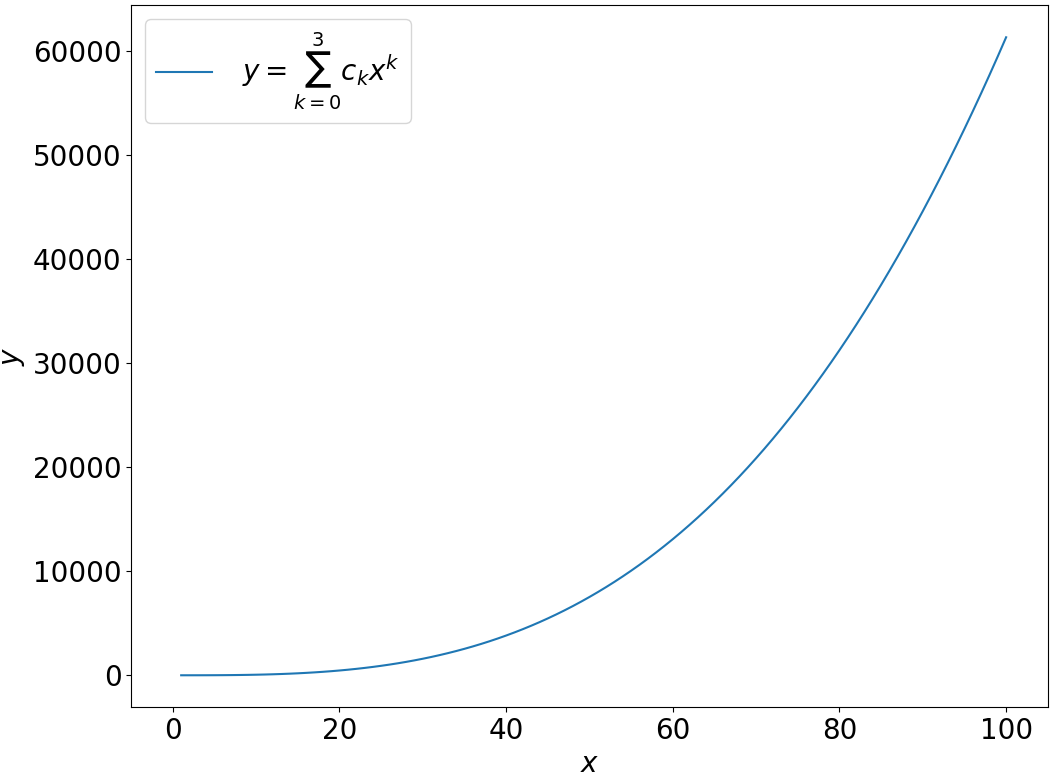
\includegraphics[width=\linewidth]{q3_N=3}
	\captionof{figure}{Plot of power series estimate of $f_{1}(x)$ for $N=3$}
	\label{q3_N=3}
\end{minipage}
\vspace{1cm}

\begin{minipage}{\textwidth}\centering
	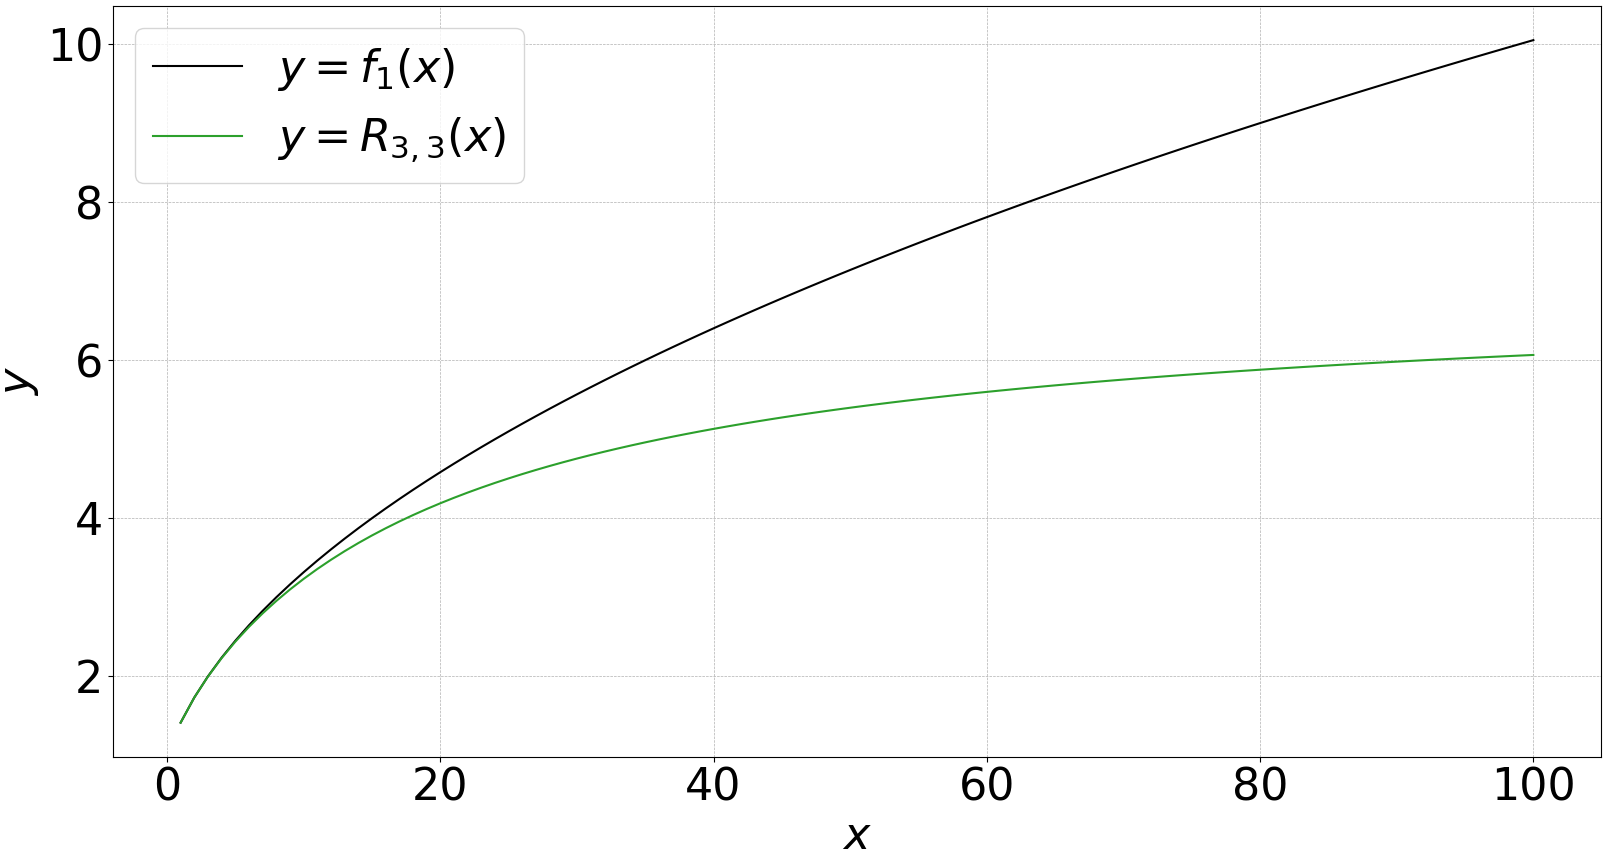
\includegraphics[width=0.8\linewidth]{q3_L=3}
	\label{q3_L=3}
\end{minipage}
\vspace{0.1cm}

\begin{minipage}{\textwidth}\centering
	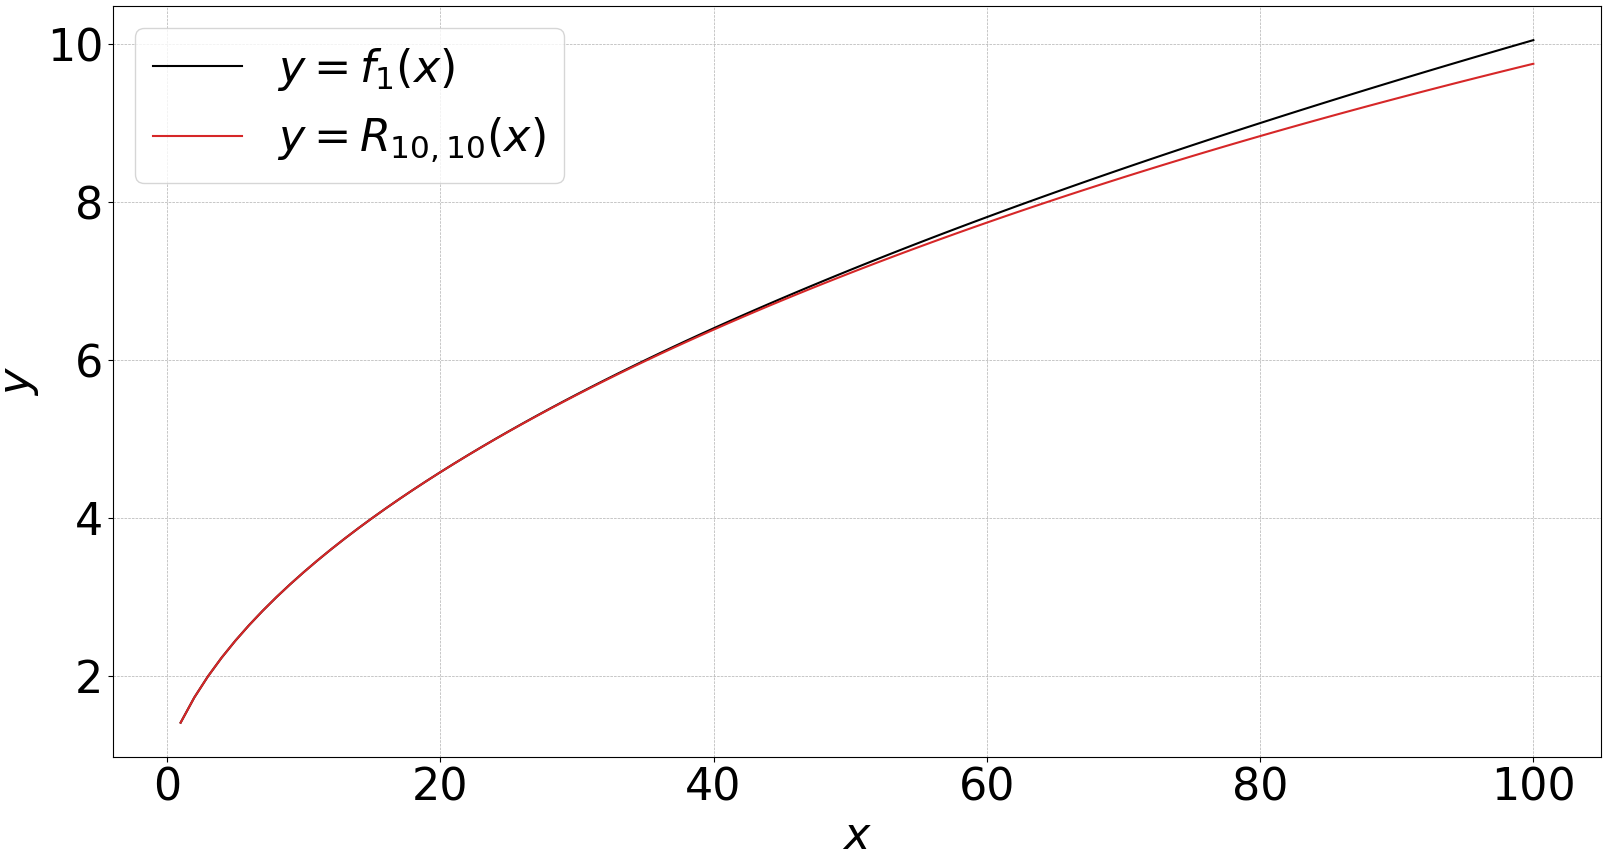
\includegraphics[width=0.8\linewidth]{q3_L=10}
	\label{q3_L=10}
\end{minipage}
\vspace{0.1cm}

\begin{minipage}{\textwidth}\centering
	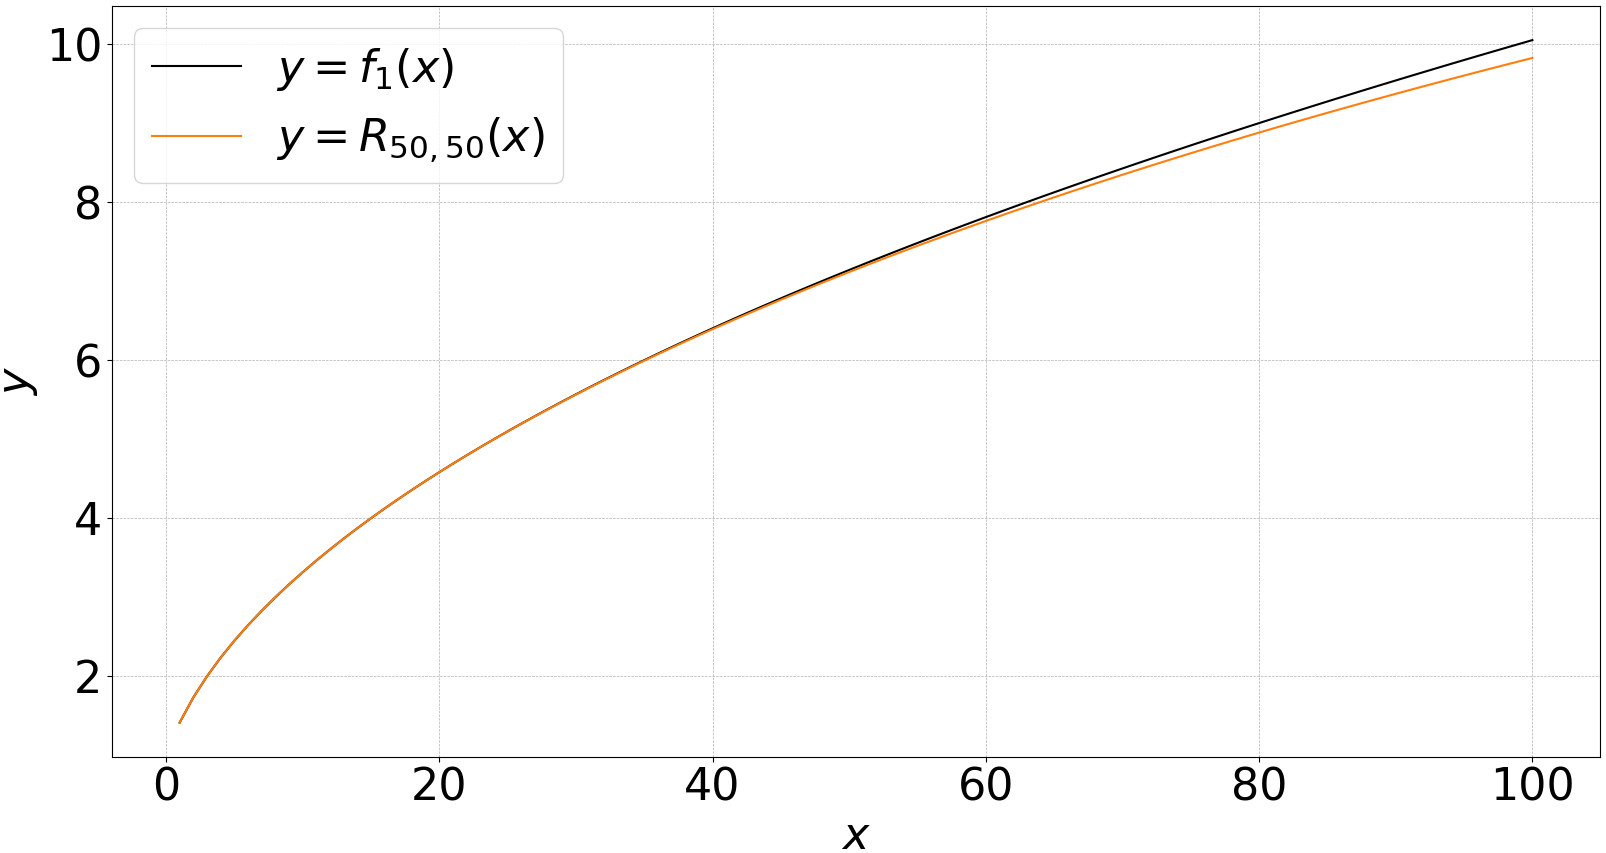
\includegraphics[width=0.8\linewidth]{q3_L=50}
	\captionof{figure}{Plots of Pad\'e approximant estimates of $f_{1}(x)$ for $L = 3, 10$ and $50$}
	\label{q3_L=50}
\end{minipage}
\vspace{0.1cm}

We can see from Figure \ref{q3_N=3} that for $N=3$, the estimate increases at a rate of $x^{N}$.
This means it diverges from $f_{1}(x)$ and for larger $N$ the estimate diverges even more quickly. This is
because of the $x^{N}$ term in the power series which becomes very large for $x > 1$.
\\

In comparion, the diagonal Pad\'e approximant with $L=3$ stays much closer to $f_{1}(x)$ than the power series
estimate. This is due to the fact that the Pad\'e approximant is a fraction so its limiting behaviour as 
$x \to \infty$ is much more similar to $f_{1}(x)$ than the power series' behaviour is. However, $L = 3$ does 
not give a good estimate in the range $1 \leq x \leq 100$. We see that for $L = 10$ and $L = 50$, we obtain
much closer estimates while the power series would only diverge further.
\\

\begin{minipage}{\textwidth}\centering
	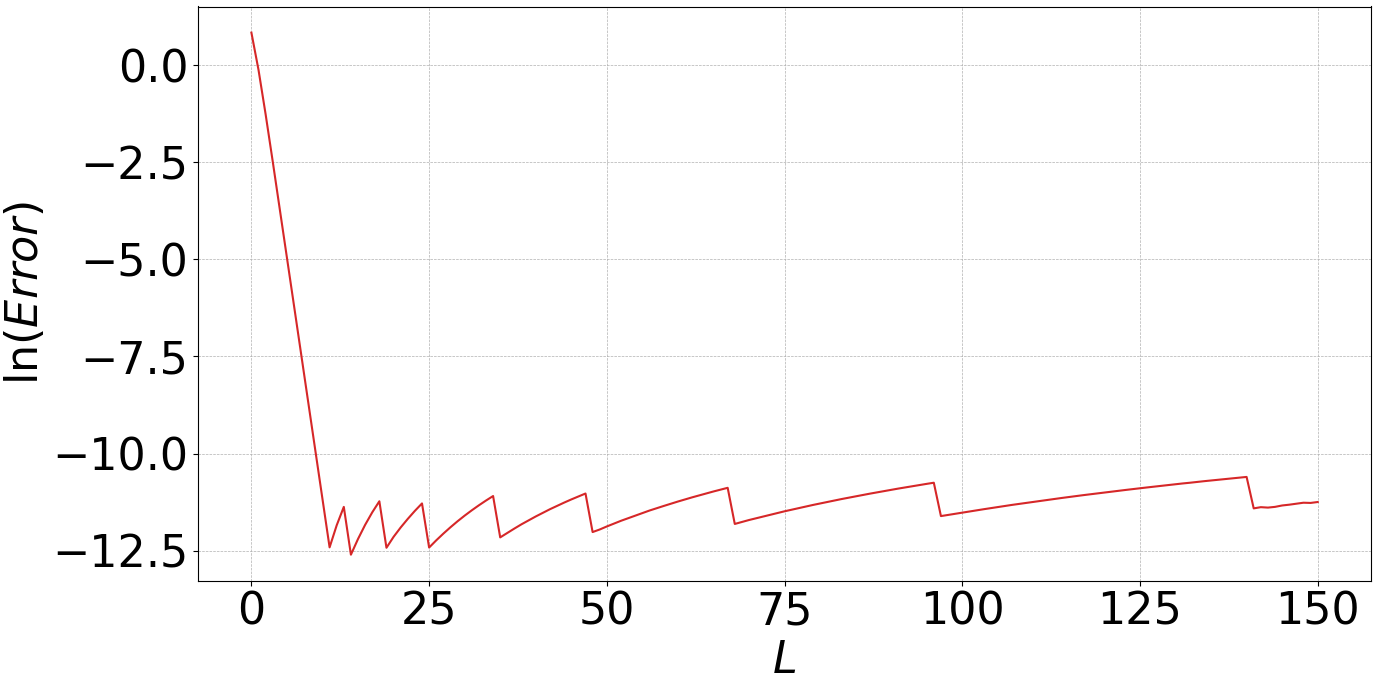
\includegraphics[width=\linewidth]{q3_fig3}
	\captionof{figure}{Plot of $L$ against $\ln(Error)$ for $x = 10$}
	\label{q3_fig3}
\end{minipage}
\vspace{1cm}

\begin{minipage}{\textwidth}\centering
	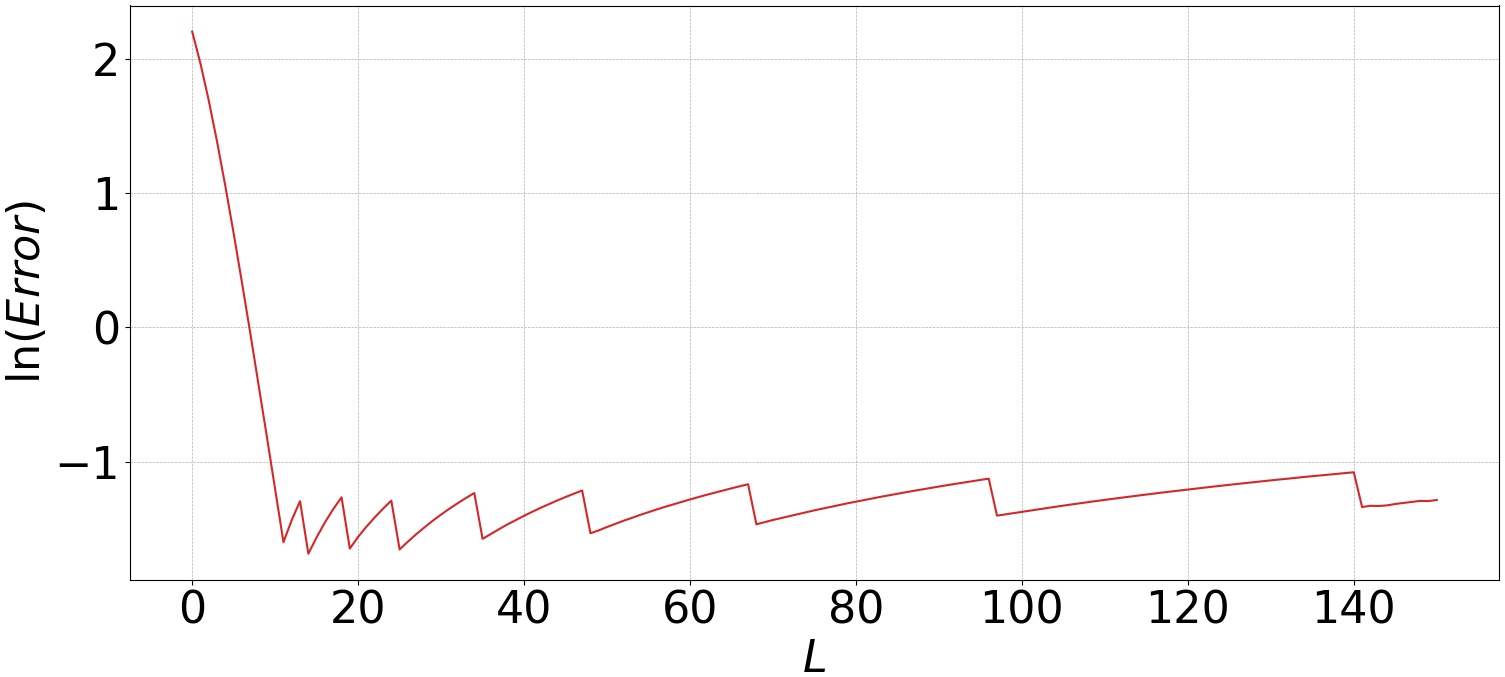
\includegraphics[width=\linewidth]{q3_fig4}
	\captionof{figure}{Plot of $L$ against $\ln(Error)$ for $x = 100$}
	\label{q3_fig4}
\end{minipage}
\vspace{1cm}

From Figures \ref{q3_fig3} and \ref{q3_fig4}, we see that the error decreases exponentially for $L \leq 11$
since the graphs are linear for this range of $L$. Beyond this range, the error remains in the same area as 
it increases and decreases in a zig-zag pattern. The reason the error stops decreasing exponentially is that
the Pad\'e approximant calculated by Program A is not accurate for large $L$ (i.e. the $q_{k}$ and $p_{k}$ 
calculated are slighly off). I know that the approximant is inacurate since it should give the same result 
as the $(2L)^{\text{th}}$ continued fraction from:
\begin{flalign*}
	\sqrt{1+x} &= 1 + \frac{ x }{ 1 + \sqrt{1+x} } && \\
	\implies \sqrt{1+x} &= 1 + \frac{ x }{ 2 + \frac{ x }{ 2 + \frac{ x }{ 2 + ...}}} &&
\end{flalign*}

Truncating this fraction after the $(2L)^{\text{th}}$ two and simplifying, we obain the diagonal Pad\'e 
approximant. The program \texttt{continued\textunderscore fraction.py} on page \pageref{continued_fraction} 
demonstrates that the results of Program A and what the approximant should be (using the continued fraction) 
are different; using $L = 15$ as an example, the error from the Pad\'e approximant is $5.03\times 10^{-6}$
while the error should be $2.77\times 10^{-8}$. This must be due to the limitations of the 64-bit float 
arithmetic used for Program A and hence explains why the error stops decreasing as $L$ is increased.
\\
%Notice that this is the same range for which the error
%decreased expnentially in Question 2 but in that case the error at $L = 11$ was the machine precision. 
% THIS IS JUST A COOINCIDENCE

% We can expect this to continue for larger $L$, meaning that we cannot expect the error to be any smaller than
% it is for $L = 14$ which is where we see a minimum on both graphs. 

% THE REASON FOR THE INACCURACY IS THAT THE PADE APPROXIMANT IS JUST WRONG. FOR EXAMPLE, THE CONTINUED FRACTION
% WHICH SIMPLIFIES INTO THE PADE APPROXIMANT GIVES THE CORRECT SOLUTION. KNOW WHAT THE CORRECT SOLUTION
% IS BECAUSE WOLFRAM ALPHA GIVES IT EXACTLY (ALTHOUGH HERE HAVE TO SAY I KNOW IT FROM CONTINUED FRACTION
% BUT WOLFRAM AND CONTINUED FRACTION GIVE THE SAME RESULT SO I KNOW CONTINUED FRACTION IS CORRECT)

Overall, we can see that the Pad\'e approximant almost converges to $f_{1}(x)$ for large $x$ despite\ 
the fact that this is outside the radius of convergence of the power series. However, there is a\ 
limitation on the accuracy of the estimate you can get where increasing the value of $L$ will not\ 
improve the result.
% ONE MORE IMPLICATION


\subsubsection*{Question 4}

I first present some graphs which give the error for different L using a diagonal approximant and
the error for different orders using the power series. This is so that the optimal such L and order
can be found for calculation across the whole range $0 \leq x \leq 20$.

\begin{minipage}{\textwidth}
	\centering
	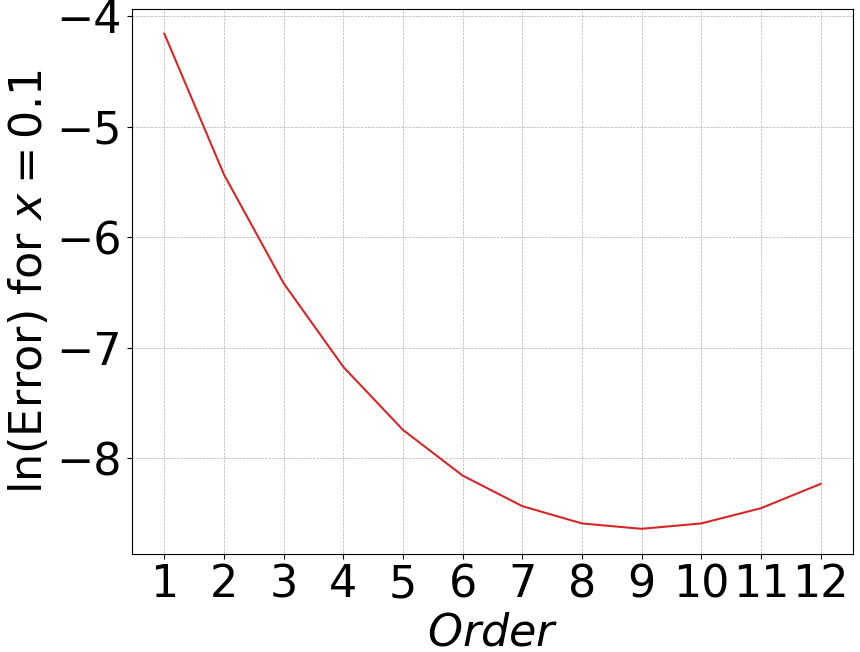
\includegraphics[width=0.49\linewidth]{q4_series_x=0.1}
	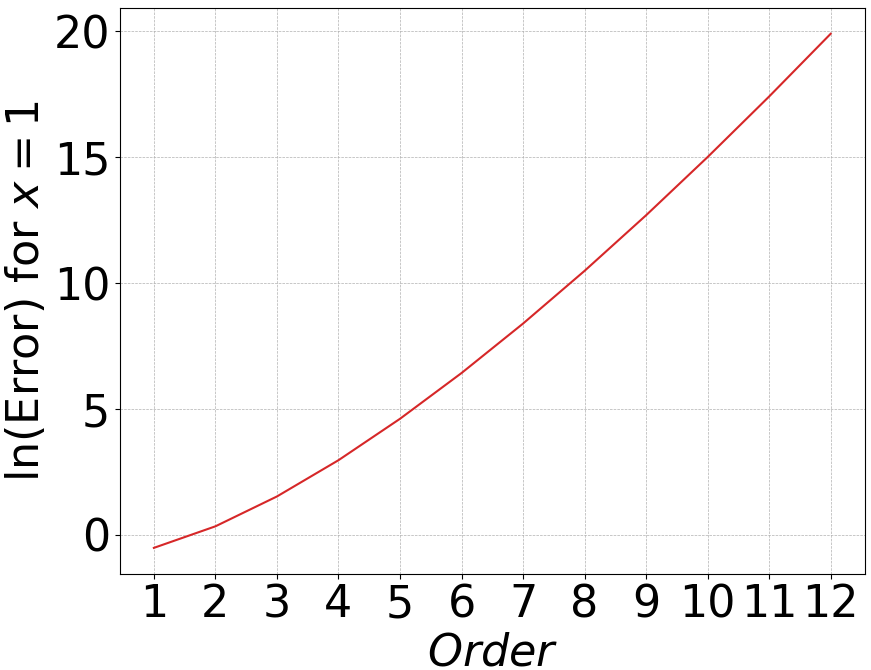
\includegraphics[width=0.49\linewidth]{q4_series_x=1}
	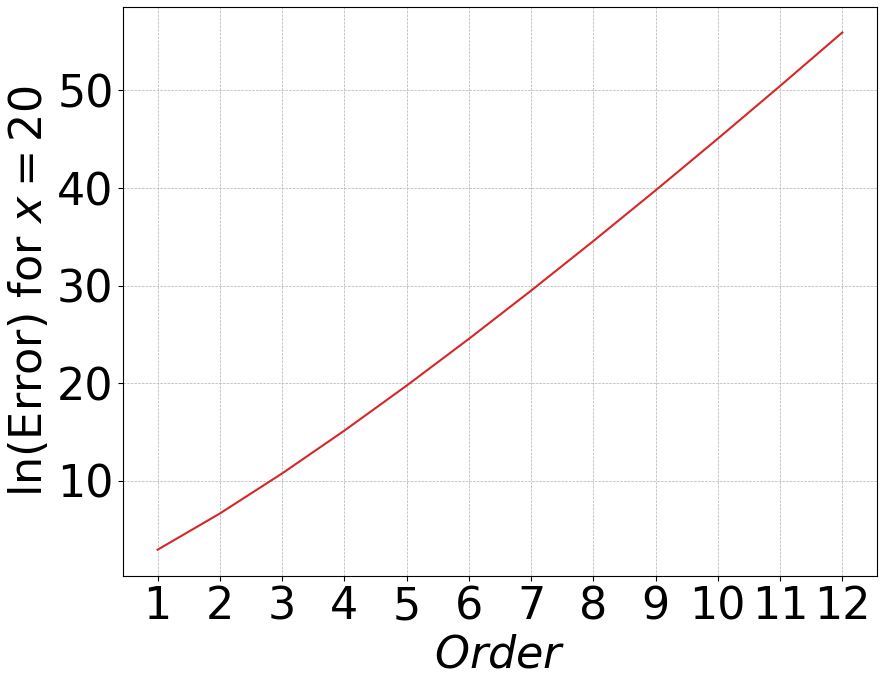
\includegraphics[width=0.5\linewidth]{q4_series_x=20}
	\captionof{figure}{Plots of power series order against $\ln(Error)$ for $x = 0.1, 1$ and $20$}
	\label{q4_series_change}
\end{minipage}
\vspace{0.5cm}

\begin{minipage}{\textwidth}
	\centering
	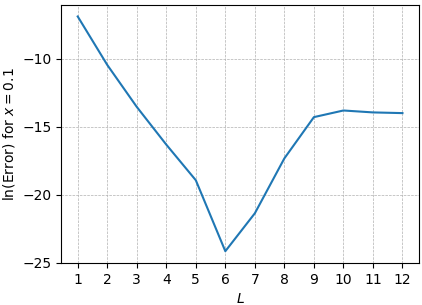
\includegraphics[width=0.49\linewidth]{q4_approx_x=0.1}
	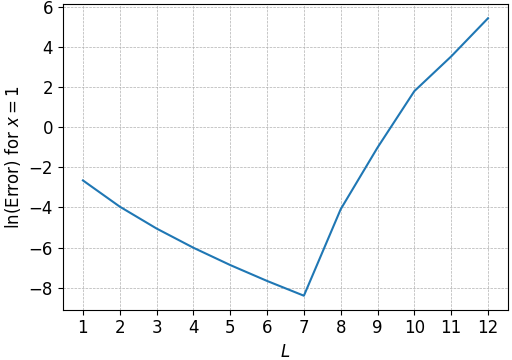
\includegraphics[width=0.49\linewidth]{q4_approx_x=1}
	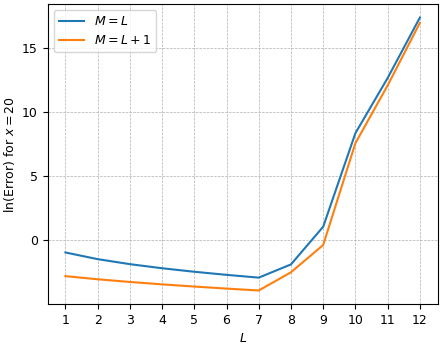
\includegraphics[width=0.5\linewidth]{q4_approx_x=20}
	\captionof{figure}{Plots of $L$ against $\ln(Error)$ for $x = 0.1, 1$ and $20$}
	\label{q4_approx_change}
\end{minipage}
\vspace{0.5cm}

From Figure \ref{q4_series_change} we can see that for large $x \geq 1$ the error of the power series
estimates diverges exponentially so the power series is not useful for any order here. On the other
hand, the graph with $x = 0.1$ demonstrates that the series gives a good estimate for much smaller x
as the $x^{n}$ terms do not diverge. In particular, the order of $9$ gives the minimum error.
\\

Figure \ref{q4_approx_change} shows that the Pad\'e approximant can give a relatively small error
for different values of $x$ in the range $[0, 20]$. The minimum error is given by either $L = 6$ or
$L = 7$ and taking the diagonal approximant.
\\

\begin{minipage}{0.45\textwidth}
	\centering
	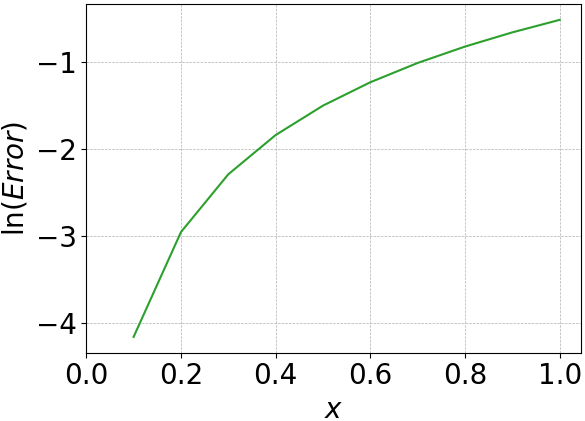
\includegraphics[width=\linewidth]{q4_series_order=1}
	\captionof{figure}{Error from the order 1 power series}
	\label{q4_series_o1}
\end{minipage}
\hspace{0.9cm}
\begin{minipage}{0.45\textwidth}
	\centering
	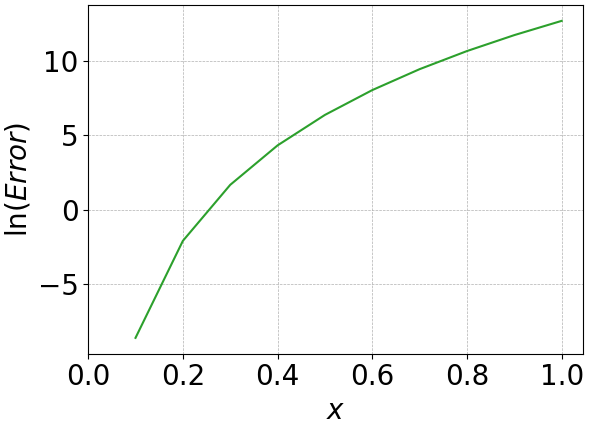
\includegraphics[width=\linewidth]{q4_series_order=9}
	\captionof{figure}{Error from the order 9 power series}
	\label{q4_series_o2}
\end{minipage}
\vspace{0.5cm}

\begin{minipage}{0.45\textwidth}
	\centering
	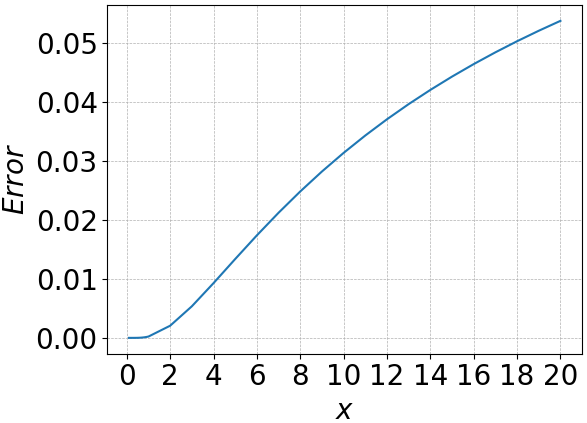
\includegraphics[width=\linewidth]{q4_approx_L=7}
	\captionof{figure}{Error of Pad\'e approximant with $L = 7$ in range the [0,20]}
	\label{q4_approx_L=7}
\end{minipage}
\hspace{0.9cm}
\begin{minipage}{0.48\textwidth}
	\centering
	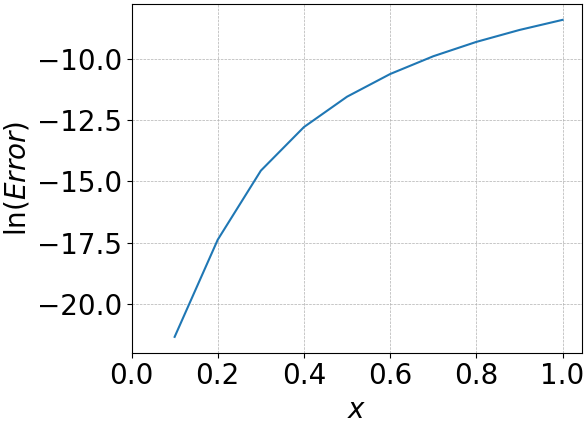
\includegraphics[width=\linewidth]{q4_approx_zoomed}
	\captionof{figure}{Error of Pad\'e approximant with $L = 7$ zoomed in on the range [0,1]}
	\label{q4_approx_zoomed}
\end{minipage}
\vspace{0.5cm}

Since the power series diverges for larger $x$, only the Pad\'e approximant is a good basis
for calculating $f_{2}(x)$ in the range $0 \leq x \leq 20$. Figure \ref{q4_approx_L=7} shows
that the error remains small up to $x=20$. In the range $0 \leq x \leq 1$, the Pad\'e approximant
approximant also gives far more accurate calculations than the power series comparing Figures
\ref{q4_series_o1}, \ref{q4_series_o2} and \ref{q4_approx_zoomed}. In addition, while the order 9
power series gives a small error for $x = 0.1$, this quickly diverges.
\\

The reason that the Pad\'e approximant is more accurate than the truncated power series is similar
to the reasoning for $f_{1}(x)$; the limiting behaviour is better because the approximant 
is a fracion and for small $x$ the power series expansion of the Pad\'e approximant is better
than the truncated power series with the matching first $L + M + 1$ terms.

\subsubsection*{Question 5}

I will display the values of $x$ at the poles and zeros of the Pad\'e approximant of $f_{1}(x)$ for 
selected $L$.\\
\underline{Poles}\\
$L = 1: ~~~ x \approx -4$\\
$L = 3: ~~~ x \approx -20.196, -2.572, -1.232$\\
$L = 10: ~~ x \approx -179.079, -20.197,~....., -1.095, -1.023$\\
\underline{Zeros}\\
$L = 1: ~~~ x \approx -1.333$\\ 
$L = 3: ~~~ x \approx -5.312, -1.636, -1.052$\\
$L = 10: ~~ x \approx -45.021, -11.511,~.....,  -1.052, -1.006$
\\

All poles and zeros are real. Additionally, there are exactly $L$ poles and zeros for $R_{L,L}(x)$ meaning
that there is one more pole and zero when $L$ is increased by one. All poles and zeros are negative, with
the least negative values approaching 1 as $L$ is increased. Meanwhile, the largest negative increases as
$L$ is increased and the remaining poles/zeros lie between this value and 1.
\\ 
ALSO ANOMALOUS POLES and ZEROS NON-REAL FOR LARGE L
\\

The Pad\'e approximant of $f_{3}(x)$ is the inverse of the Pad\'e approximant of $f_{1}(x)$. Therefore, the
poles of this approximant are the zeros of the approximant of $f_{1}(x)$ and vice versa. Hence the results
above can be used to describe their behaviour.
\\

We have the following results for $f_{4}(x)$.
% \underline{Poles}\\
% $L = 1: ~~~ x \approx -4$\\
% $L = 3: ~~~ x \approx -20.196, -2.572, -1.232$\\
% $L = 10: ~~ x \approx -179.079, -20.197,~....., -1.095, -1.023$

\vspace{0.3cm}
\begin{minipage}{\textwidth}
	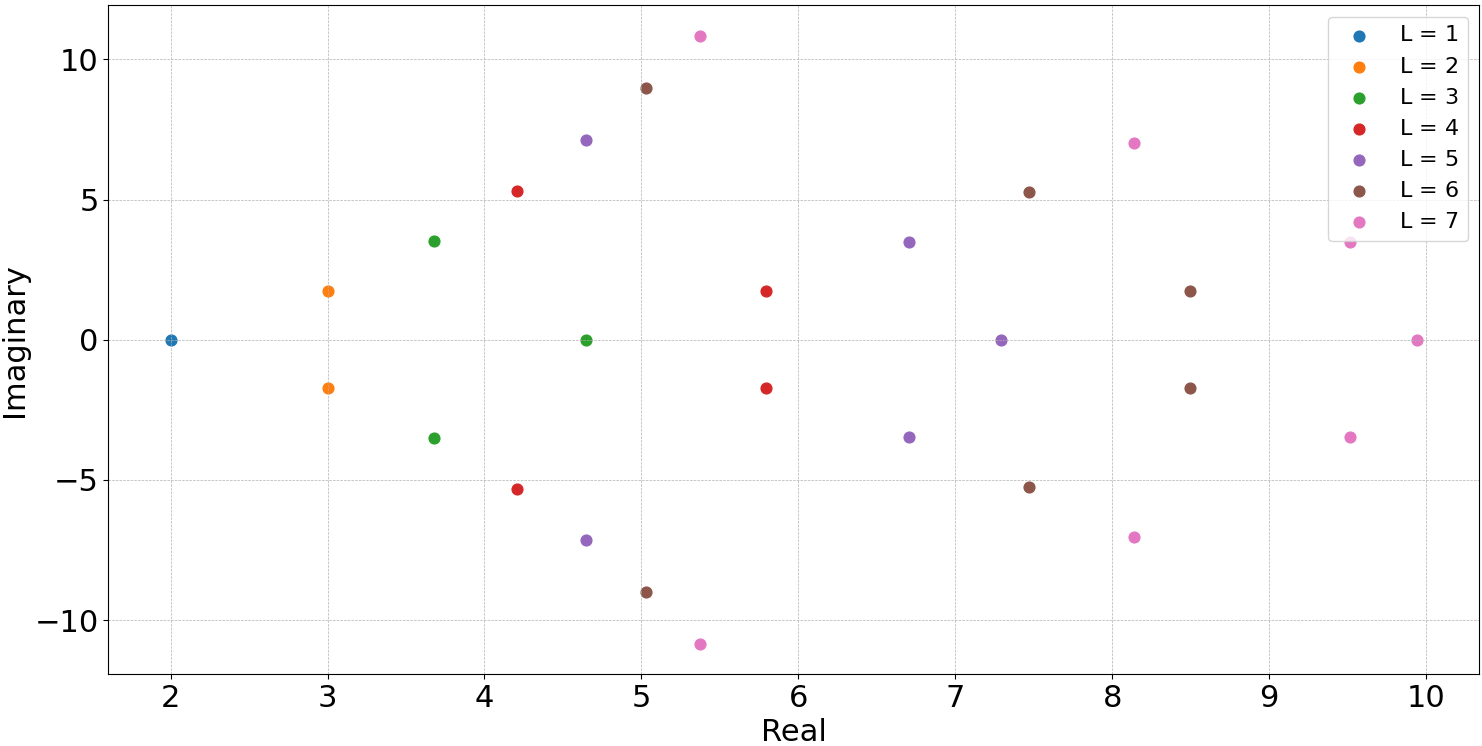
\includegraphics[width=\linewidth]{q5_fig1_poles}
	\captionof{figure}{Scatter graph showing poles of $R_{L,L}(x)$}
	\label{q5_fig1_poles}
\end{minipage}
\vspace{0.1cm}

\vspace{0.3cm}
\begin{minipage}{\textwidth}
	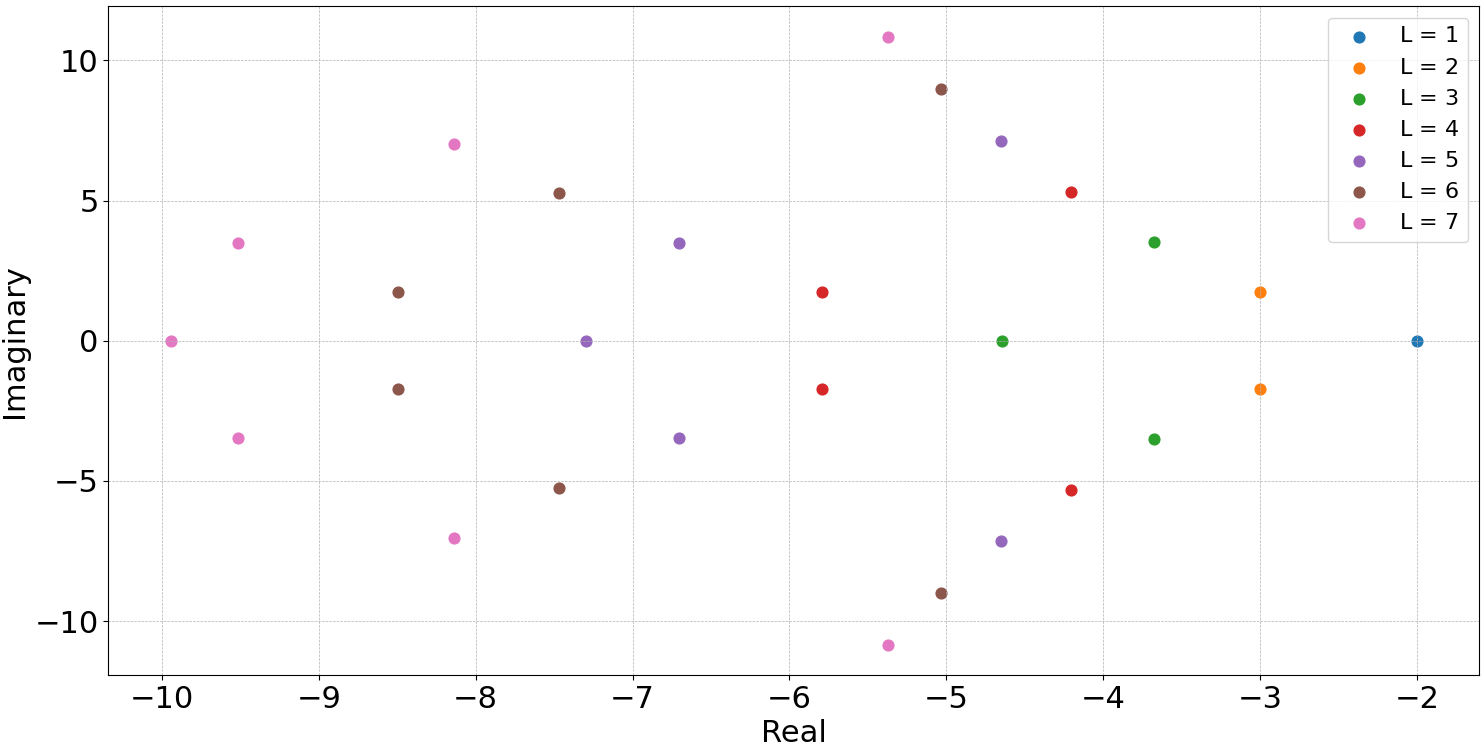
\includegraphics[width=\linewidth]{q5_fig1_zeros}
	\captionof{figure}{Scatter graph showing zeros of $R_{L,L}(x)$}
	\label{q5_fig1_zeros}
\end{minipage}
\vspace{0.1cm}

From Figures \ref{q5_fig1_poles} and \ref{q5_fig1_zeros}, we notice that there are mostly complex roots
in conjugate pairs with the magnitude increasing as $L$ increases. There are no real poles or zeros for 
$L = 2, 4 \text{ or } 6$ however there is exactly one for all odd $L$ excluding 1, and exactly two for
the remaining even $L\geq 8$.
\\

We can obtain similar graphs for $f_{5}(x)$. The number of real poles and zeros remains the same as above
apart from the fact that there are two real poles for $L = 4$ and $L = 6$. When there are real poles, 
there is always one very close to -1 and for even values of $L$ there is an additional positive real pole. 
For instance, for $L = 14$ there are poles -1.00 and 1.48. As $L$ increases above 10, additional poles 
and zeros are within a distance of 2 to the origin.
\\

For $f_{6}(x)$, there is a real pole for $L\geq 2 $ with increasingly large magnitute. For example, for 
$L = 9$ there is a pole at $x=7390.11$ and for $L=10$ there is one at $x=-22133$. This large real pole 
alternated between positive and negative values for odd and even values of $L$ respectively and seems
to increase in magnitude by a factor of approximately 3 each time $L$ is increased. There is a second
real pole for even $L$ which is just less than -2. The remaining poles tend towards 
$-\frac{1}{2} \pm \frac{\sqrt{3}}{2}$ as outline in Figure \ref{q5_fig2}.\\
\vspace{0.3cm}
\begin{minipage}{\textwidth}
	\centering
	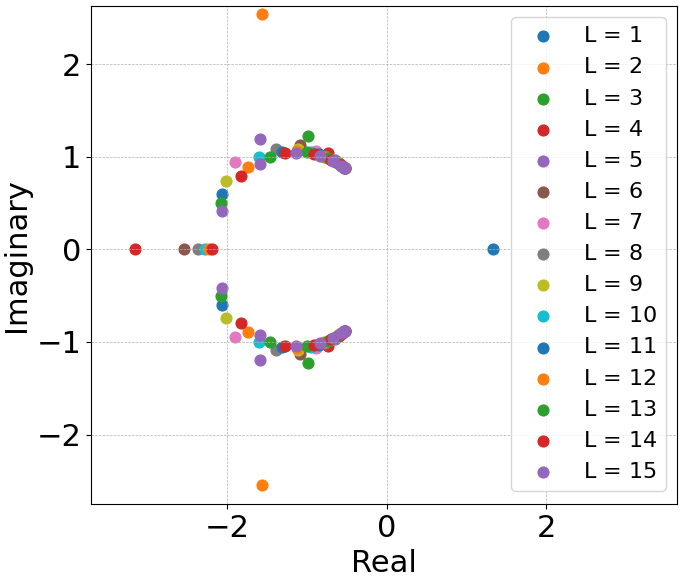
\includegraphics[width=0.6\linewidth]{q5_fig2}
	\captionof{figure}{Graph showing poles of $f_{6}$}
	\label{q5_fig2}
\end{minipage}
\vspace{0.1cm}

The zeros of $f_{6}(x)$ are positioned in an identical fashion to Figure \ref{q5_fig2} with an increasing 
number of roots approaching $-\frac{1}{2} \pm \frac{\sqrt{3}}{2}$.
\\

The least negative poles and zeros of the approximants of $f_{1}(x)$ and $f_{3}(x)$ tending to -1 corresponds
to a branch point of both functions at $x=-1$. The remaining poles and zeros can be 
considered to be lying on a branch cut along the negative real axis. PLOT or table
\\

$f_{4}(x)$ has no zeros, poles or branch points so there is no correspondence with the approximants.
$f_{5}(x)$ has a pole at $z = -1$ which corresponds to the real poles we find very close to -1 in the
approximants. Table \ref{table_1} demonstrates this in more detail. TABLE
\begin{table}[htb]
	\renewcommand{\arraystretch}{1.7}  % Stops rows being so close together
	\begin{tabular}{c|c|c|c|c|c|c|}
		\cline{2-7}
		& ~~\_\space\space\space & ~~R~~ & ~RE\space\space & ~REA\space\space & REAC\space & REACT \\\hline
		\multicolumn{1}{|c|}{\_} & 0  & 1 & 2  & 3   & 4    & 5     \\ \hline
		\multicolumn{1}{|c|}{C}   & 1  & 1 & 2  & 3   & 3    & 4     \\ \hline
		\multicolumn{1}{|c|}{CA}   & 2  & 2 & 2  & 2   & 3    & 4     \\ \hline
		\multicolumn{1}{|c|}{CAT} & 3  & 3 & 3  & 3   & 3    & 3     \\ \hline
	\end{tabular}
	\label{table_1}
\end{table}
\\

We find that $-\frac{1}{2} \pm \frac{\sqrt{3}}{2}$ are zeros and branch points of $f_{6}(x)$ which
explains why the zeros approach these values. $\infty$ is the third and final branch point so any branch
cut requires two segments. Thus the poles lying along the real axis can be considered to be lying along
a segment of a branch cut which goes from one of the finite branch points and to $\infty$ along the real 
axis.
% (Figure 16 already presented above helps to highlight this)


\pagebreak
\textbf{Program\textunderscore A.py for Programming Task}\centering\label{Program_A}
\lstinputlisting[language=Python]{C:/Users/angus/OneDrive/Documents/CATAM 7.5/Program_A.py}
\vspace{2cm}

\pagebreak
\textbf{Program\textunderscore B.py for Programming Task}\centering\label{Program_B}
\lstinputlisting[language=Python]{C:/Users/angus/OneDrive/Documents/CATAM 7.5/Program_B.py}
\vspace{2cm}

\pagebreak
\textbf{Question\textunderscore 1.py for Question 1}\centering\label{Question_1}
\lstinputlisting[language=Python]{C:/Users/angus/OneDrive/Documents/CATAM 7.5/Question_1.py}
\vspace{2cm}

\pagebreak
\textbf{Question\textunderscore 1.py for Question 2}\centering\label{Question_2}
\lstinputlisting[language=Python]{C:/Users/angus/OneDrive/Documents/CATAM 7.5/Question_2.py}
\vspace{2cm}

\pagebreak
\textbf{Question\textunderscore 2.py for Question 3}\centering\label{Question_3}
\lstinputlisting[language=Python]{C:/Users/angus/OneDrive/Documents/CATAM 7.5/Question_3.py}
\vspace{2cm}

\pagebreak
\textbf{continued\textunderscore fraction.py for Question 3}\centering\label{continued_fraction}
\lstinputlisting[language=Python]{C:/Users/angus/OneDrive/Documents/CATAM 7.5/continued_fraction.py}
\vspace{2cm}

\pagebreak
\textbf{Question\textunderscore 4.py for Question 4}\centering\label{Question_4}
\lstinputlisting[language=Python]{C:/Users/angus/OneDrive/Documents/CATAM 7.5/Question_4.py}
\vspace{2cm}

\pagebreak
\textbf{Question\textunderscore 5.py for Question 5}\centering\label{Question_5}
\lstinputlisting[language=Python]{C:/Users/angus/OneDrive/Documents/CATAM 7.5/Question_5.py}
\vspace{2cm}


\end{document}